\documentclass{article}
\usepackage{graphicx}
\begin{document}
\begin{figure}
    \centering
    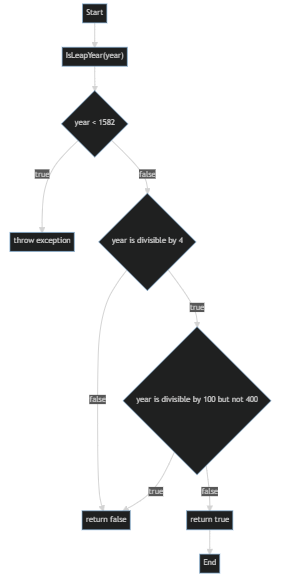
\includegraphics{Flowchart.png}
    \caption{As can be seen, the IsLeapYear method is fairly straight forward. The year has to meet 3 criteria for the method to return true: Firstly it should be divisible by 4, and secondly it should never be divisible by 100 unless it is also divisible by 400. Lastly, it should never be below the year 1582.}
\end{figure}
\end{document}
